\section{Sinusoidal Waves and Boundaries}

\subsection{Sinusoidal Waves}
We now turn our attention to a particular class of waves. Sinusoidal waves are shaped like sine/cosine functions and generally take the form $y(x, t) = A \sin (kx - \omega t)$, where we define $A$ to be the amplitude, $k$ to be the wave number, and $\omega$ to be the angular frequency. 
\begin{center}
\begin{asy}
	import graph;
	size(200);
	real shift = 0.2;
	real down = -0.2;
	real f(real x) 
	{ 
		return 3*sin(pi*x/4); 
	} 
	Label f; 
	f.p=fontsize(6); 
	draw(graph(f,0,12));
	draw((0,0)--(12, 0), linetype("8 8")); 
	draw((10, 3)--(10,0), Arrows); 
    label("$A$", (10, 3)--(10,0), E); 
    draw((2, 3.5)--(10,3.5), Arrows);
    label("$\lambda$", (10, 3.5)--(2,3.5), N); 
    
    dot((0,0), blue); dot((4,0), blue); dot((8,0), blue); dot((12,0), blue);
    dot((2,3), red); dot((6,-3), red); dot((10, 3), red); 
\end{asy}
\end{center}
We also define the wavelength $\lambda$, the period $\tau$,\footnote{usually denoted with $T$, but not to be confused with the tension $T$} and the frequency $f$.\footnote{usually denoted with $\nu$, but not to be confused with the velocity $v$} Sinusoidal waves are periodic, so the period $\tau$ is the time between the instances where the wave at a certain point is the same. The wavelength $\lambda$ is the distance between equal parts of the periodic wave (ie. between two crests or two troughs), and the frequency $f$ is the number of periods of the wave that pass by a certain point per unit time. Sinusoidal waves, by themselves are also moving with a speed $v$. \\
We can define a number of relations among these variables: 
\[
	\lambda = \frac{2\pi}{k} \quad f = \frac{\omega}{2\pi} = \frac{1}{T} \quad v = \frac{\omega}{k} = \frac{\lambda}{T} = \sqrt{\frac{T}{\mu}}
\]
Let's apply our formulas for energy from the last lecture to find the energy stored in one wavelength in a typical sinusoidal wave. Recall that the energy density $\epsilon$ is: 
\begin{align*}
\epsilon &= \frac{1}{2} \mu \left( \pdv{y}{t} \right)^2 + \frac{1}{2} T \left( \pdv{y}{x} \right)^2 \\
&= \frac{1}{2} \mu \omega^2 A^2 \cos^2 (kx - \omega t) + \frac{1}{2} T k^2 A^2 \cos^2 (kx - \omega t) \\
&= Tk^2 A^2 \cos^2 (kx-\omega t) 
\end{align*}
where this last simplification comes from noting that $Tk^2 = \mu \omega^2$ and combining terms. Integrating, we now have: 
\[
	E = \int_0^\lambda Tk^2 A^2 \cos^2 (kx-\omega t) \, dx = \frac{1}{2} TA^2k^2 \lambda = \pi TA^2 k = 2\pi^2 A^2 \mu f v 
\]
We can also find the power in this sinusoidal wave: 
\[
	P = Tk^2 A^2v \cos^2 (kx-\omega t) = T k \omega A^2 \cos^2 (kx - \omega t) = \mu \omega^2 A^2 \cos^2 (kx - \omega t) = 4\pi^2 \mu f^2 A^2 \cos^2 (kx - \omega t) 
\]
We can see from this that the maximum power in the wave is concentrated at the points where $kx - \omega t = n \pi$ for some integer $n$, which are the points that lie on the center line of the wave. These points are called the nodes of the wave (marked in blue). The points of maximum displacement in the wave are called the antinodes, and form this expression we see that the antinodes have zero energy and power instantaneously flowing out of these points (marked in red). In general, for any wave, it's worth noting that the energy (and hence, power, energy density, etc.) is always proportional to the amplitude squared. \\
It's also worth looking at the average power from this propagating wave. If we note that the average value of $\sin^2 (kx-\omega t)$ on one wavelength is $\frac{1}{2}$, we can find the average power over the wave as: 
\[
	\expval{P} = 2\pi^2 \mu f^2 A^2
\]
We can also look specifically at the contributions of kinetic and potential energy density to the energy density and power: 
\begin{align*}
\epsilon_K &= \frac{1}{2} \mu \omega^2 A^2 \cos^2 (kx - \omega t)\\
K &= \frac{1}{4} TA^2k^2 \lambda = \frac{1}{2} \pi TA^2 k = \pi^2 A^2 \mu f v  \\
P_K &= \frac{1}{2} T k \omega A^2 \cos^2 (kx - \omega t) = 2\pi^2 \mu f^2 A^2 \cos^2 (kx - \omega t) \\
\expval{P_K} &= \pi^2 \mu f^2 A^2 
\end{align*}
\begin{align*}
\epsilon_U &= \frac{1}{2} T k^2 A^2 \cos^2 (kx - \omega t)\\
U &= \frac{1}{4} TA^2k^2 \lambda = \frac{1}{2} \pi TA^2 k = \pi^2 A^2 \mu f v  \\
P_U &= \frac{1}{2} T k \omega A^2 \cos^2 (kx - \omega t) = 2\pi^2 \mu f^2 A^2 \cos^2 (kx - \omega t) \\
\expval{P_U} &= \pi^2 \mu f^2 A^2 
\end{align*}
From this, we see that the kinetic and potential energy flows are exactly the same and each contribute half of the energy. They are also in phase, meaning that they occur at the same place in each period. We will see that this is not the case for all waves. 
\subsection{Standing Waves}
In the last section, we specifically talked about propagating sinusoidal waves, which move all in one direction. We will now move to talk about standing waves, which take the form $y(x, t) = A \sin (kx) \cos (\omega t)$, and appear to oscillate in place. Standing waves appear to have their nodes and antinodes at the same positions at all times $t$. 
\begin{center}
\begin{asy}
	import graph;
	size(200);
	real shift = 0.2;
	real down = -0.2;
	real f(real x) 
	{ 
		return 3*sin(pi*x/4); 
	} 
	real g(real x)
	{
		return -3*sin(pi*x/4);
	}
	Label f; 
	f.p=fontsize(6); 
	draw(graph(f,0,12));
	Label g; 
	g.p=fontsize(6);
	draw(graph(g,0,12), linetype("4 4"));
	draw((0,0)--(12, 0), linetype("8 8")); 
	draw((10, 3)--(10,0), Arrows); 
    label("$A$", (10, 3)--(10,0), E); 
    draw((2, 3.5)--(10,3.5), Arrows);
    label("$\lambda$", (10, 3.5)--(2,3.5), N); 
    
    dot((0,0), blue); dot((4,0), blue); dot((8,0), blue); dot((12,0), blue);
    dot((2,3), red); dot((2,-3), red);
    dot((6,3), red); dot((6,-3), red); 
    dot((10, 3), red); dot((10,-3), red);
\end{asy}
\end{center}
Using the sum-to-product identities for trigonometric functions, we can decompose any standing wave as follows: 
\[
 \sin(A+B) + \sin(A-B) = 2 \sin A \cos B  
\]
\[
	\Rightarrow \sin kx \cos \omega t = \frac{1}{2} ( \sin (kx - \omega t) + \sin (kx + \omega t) ) 
\]
Standing waves are a composition of two propagating waves moving in opposite directions, but with the same wave number and angular frequency. This means that we can't use the same formulas for the power that we used in the previous section, as standing waves have components that are moving in opposite directions. However, we can compute the energy density normally: 
\begin{align*}
\epsilon &= \frac{1}{2} \mu \left( \pdv{y}{t} \right)^2 + \frac{1}{2} T \left( \pdv{y}{x} \right)^2 \\
&= \frac{1}{2} \mu \omega^2 A^2 \sin^2(kx) \sin^2(\omega t) + \frac{1}{2} T k^2 A^2 \cos^2 (kx) \cos^2 (\omega t) 
\end{align*}
Integrating over one wavelength, we can find the total energy stored in the wave:
\begin{align*}
E &= \int_0^\lambda \frac{1}{2} \mu \omega^2 A^2 \sin^2(kx) \sin^2(\omega t) + \frac{1}{2} T k^2 A^2 \cos^2 (kx) \cos^2 (\omega t) \, dx \\
&= \int_0^\lambda \frac{1}{2} T k^2 A^2 \sin^2(kx) \sin^2(\omega t) \, dx + \int_0^\lambda \frac{1}{2} T k^2 A^2 \cos^2 (kx) \cos^2 (\omega t) \, dx \\
&= \frac{1}{2} T k^2 A^2 \cdot \frac{\lambda}{2} \cdot (\sin^2 (\omega t) + \cos^2 (\omega t)) \\
&= \frac{1}{4} Tk^2 A^2 \lambda = \pi^2 A^2 \mu f v
\end{align*}
Notice that the energy in a standing wave is half of that in a propagating wave, and one fourth of the expected energy from two propagating waves. This is due to the interference of the two propagating waves canceling each others' energy contributions. \\
We can also look at the power density and the kinetic and potential energy contributions to the power density. Recall that the power density $p$ is: 
\[
	p = T \pdv{}{x} \left[\pdv{y}{x} \cdot \pdv{y}{t} \right] = \pdv{\epsilon}{t} 
\]
First, the overall power density contribution: 
\begin{align*}
	p &= T \pdv{}{x} \left[k A \cos (kx) \cos (\omega t) \cdot - \omega A \sin (kx) \sin (\omega t) \right] \\
	&= -\frac{1}{4} Tk\omega A^2 \pdv{}{x} (\sin (2kx) \sin (2\omega t)) \\
	&= -\frac{1}{2} Tk^2 \omega A^2 \cos (2kx) \sin (2\omega t)
\end{align*}
Looking at the the contributions from the kinetic and potential parts: 
\begin{align*}
	p_K = \pdv{}{t} \left[ \frac{1}{2} \mu \left(\pdv{y}{t} \right)^2 \right] &= \mu \pdv{y}{t} \pddv{y}{t} \\
	&= \mu \cdot -\omega A \sin (kx) \cos (\omega t) \cdot -\omega^2 A \sin(kx) \sin (\omega t) \\
	&= \frac{1}{2} \mu \omega^3 A^2  \sin^2 (kx) \sin (2 \omega t) \\
	&= \frac{1}{2} Tk^2 \omega A^2 \sin^2 (kx) \sin (2\omega t) 
\end{align*}
\begin{align*}
	p_U = \pdv{}{t} \left[ \frac{1}{2} T \left(\pdv{y}{x} \right)^2 \right] &= T \pdv{y}{x} \mpddv{y}{x}{t} \\
	&= T \cdot -k A \cos (kx) \sin (\omega t) \cdot k\omega A \cos(kx) \cos (\omega t) \\
	&= -\frac{1}{2} Tk^2 A^2 \omega  \cos^2 (kx) \sin (2 \omega t)
\end{align*}
By conservation of energy, the two expressions for potential and kinetic power density are expected to (and in fact, do) combine to make total power density, but they are obviously not the same expression. The locations of maximum kinetic power density occur when $kx = \frac{\pi}{2} + \pi n $ (the antinodes), whereas the locations of maximum potential energy occur when $kx = \pi n$ (the nodes). This indicates that the distributions of kinetic and potential energy are out of phase by $\frac{\pi}{2}$, unlike that of the propagating wave. 
\subsection{Boundaries and Medium Changes}
When a mechanical wave hits a rigid boundary, the wave is reflected back (which can be seen from demonstrations). What happens when a propagating wave moves between mediums of different densities? 
\begin{center}
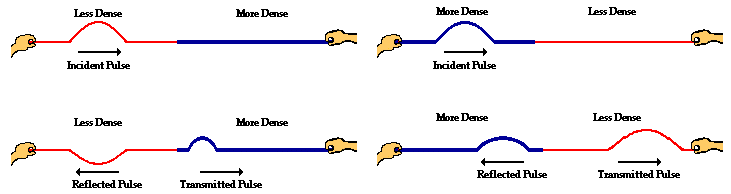
\includegraphics[scale=0.8]{images/waves/mediumchange.png}\\
\end{center}
As seen, when a propagating wave is incident on this boundary, a wave is transmitted through to the other medium, but a wave is also reflected back into the first medium. If we let the mediums have different mass densities $\mu_1$ and $\mu_2$ but with constant tension in the medium, the velocities will obviously be different. However, the frequency of all the waves will be constant - note that if $f$ periods of the wave move through the boundary, exactly $f$ periods will have to leave it - hence, the angular frequencies and frequencies of all the waves will be the same, but everything associated with length will be different between the two mediums. With this in mind, we can describe the net waves in each of the two mediums as the following: 
\[
	y_1(x, t) = A_I \sin (k_1 x - \omega t) + A_R \sin (k_1 x - \omega t) 
\]
\[
	y_2(x, t) = A_T \sin (k_2 x - \omega t) 
\]
where $k_i$ are the wave numbers of the wave in the first/second mediums, and $A_I$, $A_R$, and $A_T$ are the amplitudes of each of the incident, reflected, and transmitted waves, respectively. If we assume that the waves are continuous and differentiable at the boundary ($x=0$), we can obtain the following expressions for the amplitudes of the reflected and transmitted wave in terms of the amplitude of the incident wave: 
\[
	A_R = \frac{k_1 - k_2}{k_1 + k_2} A_I = \frac{v_2 - v_1}{v_1+ v_2} A_I \quad A_T = \frac{2k_1}{k_1 + k_2} A_I = \frac{2v_2}{v_1+v_2} A_I
\]
From this we see that if the speed of the wave in the second medium is lesser than that in the first (meaning that the medium is more dense), the reflected wave will have a negative amplitude, ie. the reflected wave will be inverted. In general, while we only derived this for sinusoidal waves, if a general incident wave is moving from a less dense to a more dense medium, the reflected wave will be inverted. \\
